\documentclass{article}
\usepackage[utf8]{inputenc}
\usepackage{amsmath}
\usepackage{xcolor}
\usepackage[top=2cm, bottom=2cm, left=2cm, right=2cm]{geometry}
\setlength\parindent{0pt}

\usepackage{listings}
%\usepackage{color}
\usepackage{graphicx}
\usepackage{float}
\usepackage{caption}

\usepackage{verbatim}
\let\oldv\verbatim
\let\oldendv\endverbatim

%\userpackage{minted}

\definecolor{dkgreen}{rgb}{0,0.6,0}
\definecolor{gray}{rgb}{0.5,0.5,0.5}
\definecolor{mauve}{rgb}{0.58,0,0.82}
\definecolor{light-gray}{gray}{0.95}


\lstset{frame=tb,
  language=Java,
  aboveskip=6mm,
  belowskip=6mm,
  showstringspaces=false,
  columns=flexible,
  basicstyle={\small\ttfamily},
  numbers=none,
  numberstyle=\tiny\color{gray},
  keywordstyle=\color{blue},
  commentstyle=\color{dkgreen},
  stringstyle=\color{mauve},
  breaklines=true,
  breakatwhitespace=true,
  tabsize=3,
  backgroundcolor=\color{light-gray},
  language=Matlab
}

%\usepackage{natbib} replaced by line below to make refernces work
\usepackage[square,sort,comma,numbers]{natbib}
\usepackage[nottoc,numbib]{tocbibind} %to get references in table of contants
\usepackage{graphicx}

\usepackage{bm}

\usepackage{hyperref}
\hypersetup{
	colorlinks,
	citecolor=black,
	filecolor=black,
	linkcolor=black,
	urlcolor=black
}

\usepackage{mdframed}
\usepackage{lipsum} % for creating dummy text
\mdfdefinestyle{MyFrame}{%
	linecolor=black,	
	backgroundcolor=gray!20!white,
	skipbelow = 8mm,
	skipabove = 8mm}

\usepackage{scrextend}

\usepackage{multimedia}
\usepackage{media9}

\title{Fys4150\\Project 3\\ }
\author{Peter Killingstad and Karl Jacobsen\\
\\
\url{https://github.com/kaaja/fys4150}}
\begin{document}
	
\maketitle



\section*{Note to instructurs about Github repository}
If the above Github-link does not work, it is eighter because you have not yet accepted our invite to the repository, or you have not yet provided us with an e-mail adress available at Github so that we can invite you. The Github user you will be invited from is "kaaja". If the latter applies to you, please send us an e-mail with an e-mailadress available in Github or your Github username so that we can send you an invite. Our e-mailadresses: peter.killingstad@hotmail.com, karljaco@gmail.com.



\section*{Abstract}
Systems of 2nd order ordinary differential equations (ODEs), describing planetary motion, are scaled and reduced to 1st order ODEs. The equations are discretized using forward Euler's method and the Velocity Verlet method, and implemented in C++ by use of classes and class inheritance. The methods is shown to involve the same number of FLOPS. Velocity Verlet is shown to be the only method the preserves energy and angular momentum, and is also higher in convergence rate order compared to forward Euler. Both methods produces reasonable planetary orbits in a two body system consisting of the sun and the earth. The velocity Verlet method reproduces exact terminal velocities for the earth, under different assumptions on the gravity force, and also gives reasonable results in a three body system both with a stationary and non-stationary sun is modelled. The full solar system is well approximated with Velocity Verlet, and the observed perihelion precession of Mercury around the sun is reproduced by adding a relativistic correction in the gravitational force.


\section{Introduction}
Multibody systems governed by coupled 2nd order ordinary differential equations (ODEs) appear several places in physics, among other places in mechanics and astrophysics. Systems like these can be simplified by variable subsitution, leading to a larger system of only 1st order ODEs. This technique is demonstrated and applied here.\\

Often the more general a method is, the more useful it is. In this project, which deals with planetary orbits, the equations are scaled to astronomical units. In addition to making the equations easier to work with, the scaling also makes the equations and their solutions more general and potentially applicable to other physical problems without the need to do large changes to the computer programs.\\

Solving large systems like these cannot be done analytically, and must be done numerically. Several methods are available for calculating derivatives that appears in the equation system. Knowledge about the properties of the different methods is crucial for getting quality solutions. There are several examples where lack of knowledge about numerical methods has led to dissasters in the real world. In this project we use the forward Euler method and Velocity Verlet method, and it is shown that the Forward Euler method do not obey basic physical properties such as energy and angular momentum preservation. Also it is shown that the speed of convergence of the Velocity Verlet method is twice that of Forward Euler.\\

Working with many equations on the computer, can increase the probability of errors lik e.g. typing errors dramatically. Methods that reduces the probability of such errors are essential for efficient and correct solutions. In physical systems like we are dealing with here, coupled 1st order ODE systems, most of the equations are almost identical. A perfect programming method for dealing with such cases are classes. With classes on typically writes many equations that is almost identical only once. This reduces the probability of typing errors considerably! Classes is used extensively in this project.\\

In this project we will deal with some special situations, like introduction of a relativistic correctional term to the gravitational force on Mercury (for calculation of the periihelion precession) and other alternative gravitational forces. Introduction of such modifications can be dealt with more smoothly, compared to adding lots of if-tests inside the classes, by utlizing class inheritance. With class ineritance, one simply construct new classes that inherits all the property of the old classes and then make simple changes to new class. This method potentially increases the readability and generality of the code, the last part implying that it can be used easier with other problems.\\

It is easy to lose control of where problems occours and how the different parts of the program works when solving large systems. Solving the full problem directly one quickly ends up with problems localizing errors, since it is hard to find errors in large systems. A step-wise implementation, incorporating only parts of the system at a time and checking different aspects at the different steps, increases the model users knowledge about the full program and system. This step wise method is implemented in this project. First a two-body system with only the sun and the earth, where the sun is stationary, is solved. On this system several things are tested: The performance of the solversm and the escape velocity for different gravitational forces. Then a three-body system is introduced, where checking for the effects of the mass of the third planet on the orbits. Finally a real center of mass system with a moving sun is introduced in the three body system, before the full solar system is simulated. \\

The next section of the report describes the equations and shows the scaling of these, in addition to describing the main idea of our class setup. The proceeding section includes all results, while the final section deals with conlcusions and discussion of limitations.


\section{Theory}

\subsection{Order reduction and differentiation methods}
Lets describe the general procedure for reducing a 2nd order ODE to a 1st order system of ODEs. Say we have an equation describing Newton's 2nd law:

\begin{equation}
F/m = a = \frac{d^2}{dx^2} = -kx
\end{equation}

Now make the "substitutions" $\frac{d^2x}{dt^2} = v$ and $v = \frac{dx}{dt}$ to get the system

\begin{subequations}
	\begin{align}\label{eq:dxdt}
	\frac{dx}{dt} &= v
	\end{align}
	
	\begin{align}
	\frac{dv}{dt} &= \frac{d^2x}{dt^2}\\
	 &= \frac{F}{m}\label{eq:dvdt}
	\end{align}
\end{subequations}

In the above the 2nd order ODE is reduced to the system (\ref{eq:dxdt}) and (\ref{eq:dvdt}). Actually, this method can be used to reduce any higher order equation to a system of 1st order ODEs! The solar system is described with Newton's 2nd law, so the reduction of order for the ODEs for the solar system follows the same recepie as listed above.\\

Now for the numerical methods, forward Euler and Velocity Verlet. Both these methods are derived from Taylor polynomials. The strength of these polynomials is that one has control over the order of the truncation error, the error one gets by truncating the Taylor series to get the wanted approximation. \\

For the forward Euler method, a Taylor expansion around the point $x + h$ is done for $x$ and $v$, and one obtain the discretized system

\begin{subequations}
	\begin{align}
		x_{i+1} = x_i + hv_i + \mathcal{O}(h^2)\label{eq:fev}
	\end{align}
	
	\begin{align}
		v_{i+1} = v_i + ha_i + \mathcal{O}(h^2)\label{eq:fea}
	\end{align}
\end{subequations}

We see from (\ref{eq:fev}) and (\ref{eq:fev}) that the truncation error is of order $h^2$. However, the above is repeated $N$ times, there are $N$ time steps, to get the full solution. Since $h$ is proprtional to $N^{-1}$ ($h = T/N$), the global error goes like $\mathcal{O}(h)$. The forward Euler method is conditionally stable, meaning that is stable only for certain $\Delta t$.\\

The velocity Verlet method is constructed in the same way as the forward Euler method, apllying Taylor polynomials. However, a more clever manipulation of the Taylor polynomials is applied, and one ends with

\begin{subequations}
	\begin{align}
	v_{i+1} = v_i + h/2(a_{i+1} + a_i + \mathcal{O}(h^3)\label{eq:vvv}
	\end{align}
	
	\begin{align}
	x_{i+1} = x_i + hv_i + \frac{h^2}{2} a_i + \mathcal{O}(h^3)\label{eq:vvx}
	\end{align}
	
	\begin{align}
	a_i = F_i/m\label{eq:vva}
	\end{align}
\end{subequations}

In the above one must update position before velocity, since we need the acceleration on the current and next step to get the velocity. Calcuating x first, we can insert this into the equation for a, and then we calculate v. We observe that the truncation error, and hence the also the global error, is one order higher compared to forward Euler. This method is unconditionally stable, meaning it is stable for all $\Delta t$. In addition, this method conserves energy.

\subsection{The solar system equations}
We describe the solar system by Newton's 2nd law assuming circular orbits and Newton's gravitational law, which for two objects are

\begin{equation}
F_G = M_{earth}\frac{v^2}{r}\label{eq:newtonCircle}
\end{equation}

\begin{equation}
F_G = \frac{GM_{sun}G_{earth}}{r^2}\label{eq:newtonGravity}
\end{equation}

Dividing both equations above by $M_{Earth}$ gives

\begin{equation}
a = \frac{v^2}{r}\label{eq:newtonCircle2}
\end{equation}

\begin{equation}
a = \frac{GM_{sun}}{r^2}\label{eq:newtonGravity2}
\end{equation}


Now we scale the equatons to Astronomical units, and get $v = \frac{2\pi r}{T} = \frac{2\pi Au}{Yr}$. Inserting this scaling into the above system gives

\begin{equation}
a = \frac{2^2 \pi^2 Au^2}{Au\;Yr^2}\label{eq:newtonCircle3}
\end{equation}

\begin{equation}
a = \frac{GM_{sun}}{Au^2}\label{eq:newtonGravity3}
\end{equation}

Setting the above two equations equal and solving for $GM_{sun}$ gives

\begin{equation}\label{eq:GMSun}
GM_{Sun} = 4 \pi^2 (Au)^3/Yr^2
\end{equation}

Now we can insert (\ref{eq:GMSun}) into (\ref{eq:newtonGravity2}) to get

\begin{equation}
a = -\frac{4 \pi^2}{r^2}
\end{equation}

For the x-component we get
\begin{subequations}
	\begin{align}\label{eq:ax}
		a_x &= -\frac{4 \pi^2}{r^2} \cos(\theta)\\
		&= -\frac{4 \pi^2}{r^2 r} r\cos(\theta)\\
		&= -\frac{4 \pi^2}{r^3} x
	\end{align}
\end{subequations}

The same type of calculation gies the y-component. \\

The next step is to add a planet to the system. This will add a new force between earth and the new planet, in addition to the force between the sun and the planets. The force between earth and the new planet will be of the exact same kind as the force between earth and sun, given in (\ref{eq:newtonGravity}), and the x accleration term (\ref{eq:ax}) for the earth will now be

\begin{equation}\label{eq:3rdPlanet}
a_x = -\frac{4 \pi^2}{r_{earth,sun}^3} (x_{earth}-x_{sun}) - \frac{4 \pi^2 \frac{M_{jupiter}}{M_{sun}}}{r_{earth,jupiter}^3}(x_{earth}-x_{jupiter}),
\end{equation}

where we see that the only difference between the two terms are the mass-factor, which in the earth-sun term is one. Now Jupiter will have the same kind of expression as above, only with Jupiter instead of earth in the subscripts. Note the similarity! Adding more planets happens in exactly the same way, nothing new happens! Also we note that the 2nd term will be equall for Jupiter and earth, which potentially can be taken advantage of when solving the equaions numerically. 


\section{Results}
Before turning to the results, we give a short overview of our class implementation.

\subsection{Class implementation}
Insert a simple figure that contains boxes of the different classes and their inouts, and arrows between boxes.

\subsection{Forward Euler versus Velocity Verlet}
The below figures show the results for the x and y-positions as functions of time, forward Euler to the left and Velocity Verlet to the right. 


\begin{minipage}{.49\textwidth} 
	\begin{figure}[H]
		\centering
		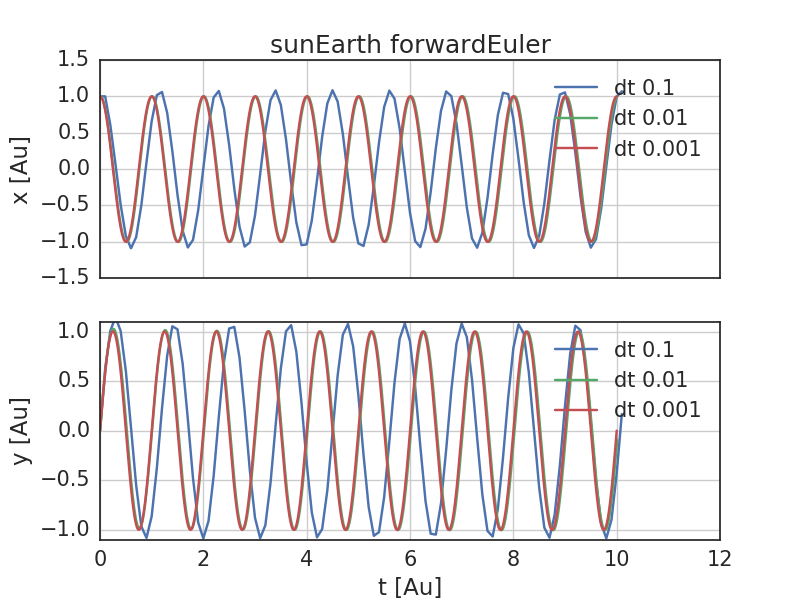
\includegraphics[width=0.99\textwidth]{/home/karl/doc/subj/att/fys4150/project3/resultsKeep/plots/sunEarthTimesForwardEuler.png}
		\caption{Sun-Earth system. Effect of $\Delta t$ over a 10 year period. \\ \textit{The Forward Euler method seems to converge for the two smallest $\Delta t$}}
		\label{1}
	\end{figure}
\end{minipage}\hfill
\begin{minipage}{.49\textwidth} 
	\begin{figure}[H]
		\centering
		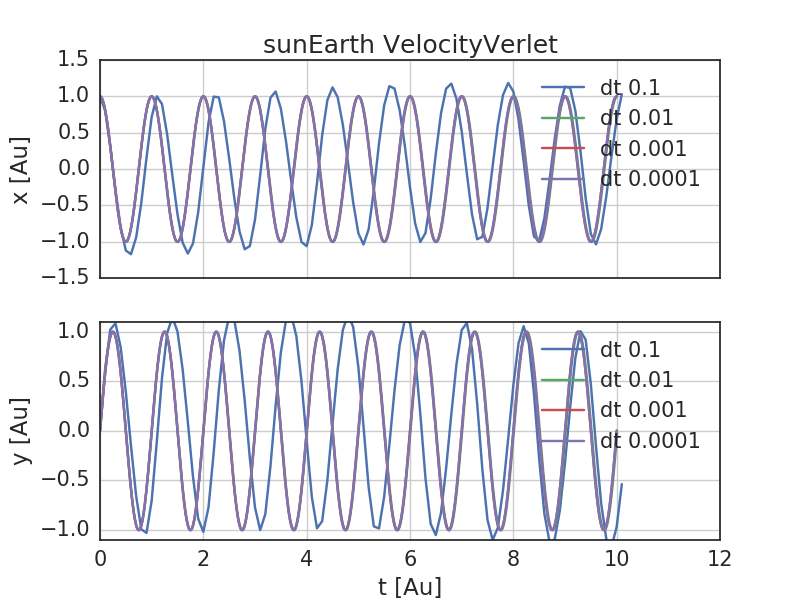
\includegraphics[width=0.99\textwidth]{/home/karl/doc/subj/att/fys4150/project3/resultsKeep/plots/sunEarthTimesVelocityVerlet.png}
		\caption{Sun-Earth system. Effect of $\Delta t$ over a 10 year period. \\ \textit{The Velocity verlet method seems to converge faster than Forward Euler}}
		\label{1}
	\end{figure}
\end{minipage}\hfill
\vspace{2ex}

As can be seen of the figures above, both methods converges when $\Delta t$ is lowered.  Also the Velocity Verlet method seems to converge faster.\\

The next two sets of figures shows the orbits for different $\Delta t$ for the two methods.

\begin{minipage}{.49\textwidth} 
	\begin{figure}[H]
		\centering
		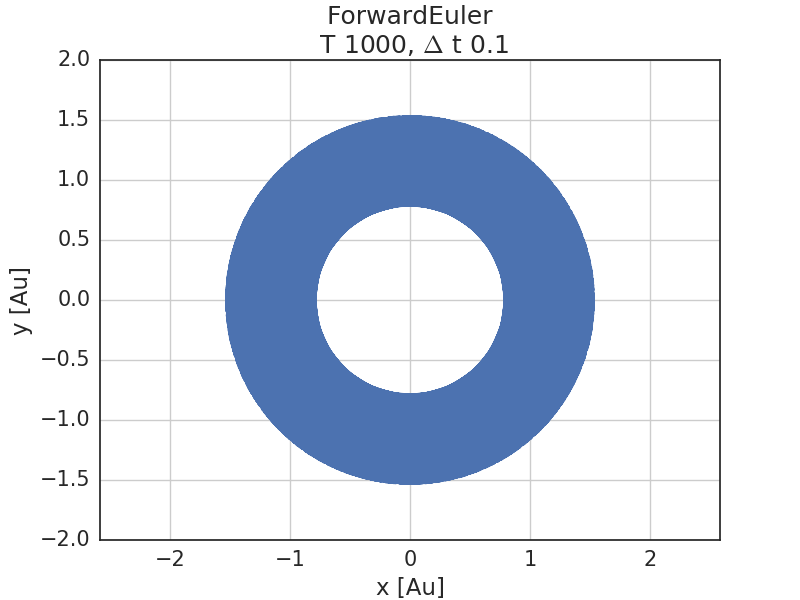
\includegraphics[width=0.99\textwidth]{/home/karl/doc/subj/att/fys4150/project3/resultsKeep/plots/sunEarthfinalTime1000N10000ForwardEuler.png}
		\caption{Sun-Earth system. Forward Euler. 1 000 years \\ \textit{Non-circulat orbits when time step is large.}}
		\label{1}
	\end{figure}
\end{minipage}\hfill
\begin{minipage}{.49\textwidth} 
	\begin{figure}[H]
		\centering
		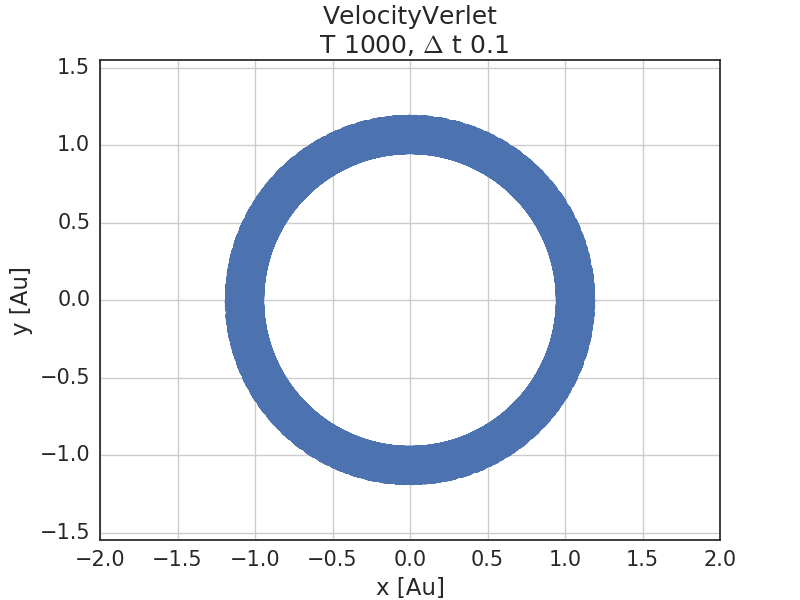
\includegraphics[width=0.99\textwidth]{/home/karl/doc/subj/att/fys4150/project3/resultsKeep/plots/sunEarthfinalTime1000N10000VelocityVerlet.png}
		\caption{Sun-Earth system. Velocity Verlet. 1000 years. \\ \textit{Large time step gives bad solutions also for Velocity Verlet.}}
		\label{1}
	\end{figure}
\end{minipage}\hfill
\vspace{2ex}

\begin{minipage}{.49\textwidth} 
	\begin{figure}[H]
		\centering
		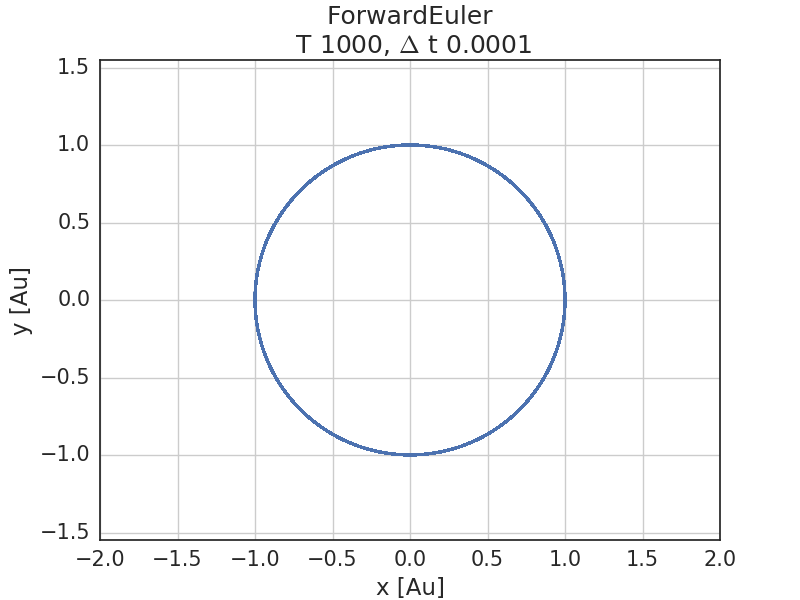
\includegraphics[width=0.99\textwidth]{/home/karl/doc/subj/att/fys4150/project3/resultsKeep/plots/sunEarthfinalTime1000N10000000ForwardEuler.png}
		\caption{Sun-Earth system. Forward Euler. 1 000 years. \\ \textit{For $\Delta t = 0.0001$, the forward Euler seems to give circular orbits, but we can see that the solution changes.}}
		\label{1}
	\end{figure}
\end{minipage}\hfill
\begin{minipage}{.49\textwidth} 
	\begin{figure}[H]
		\centering
		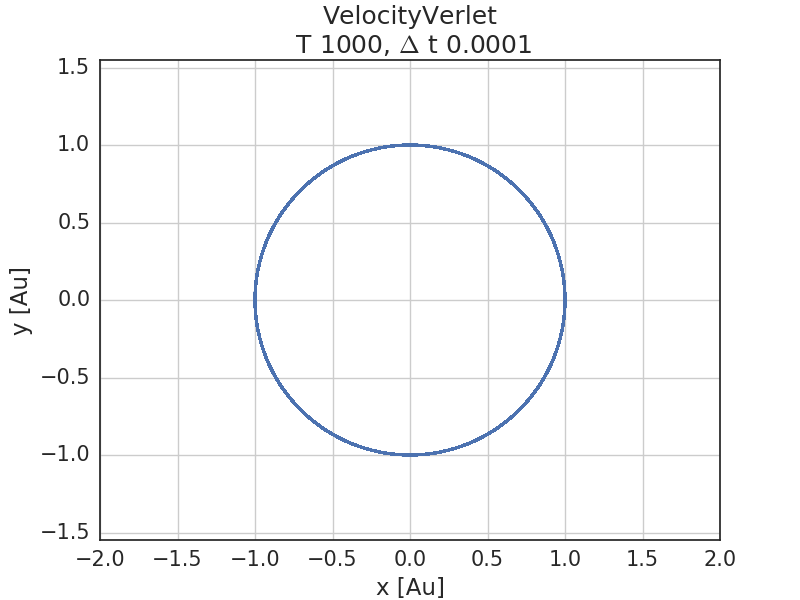
\includegraphics[width=0.99\textwidth]{/home/karl/doc/subj/att/fys4150/project3/resultsKeep/plots/sunEarthfinalTime1000N10000000VelocityVerlet.png}
		\caption{Sun-Earth system. Velocity Verlet. 1 000 years. \\ \textit{The solution looks similar to Forward Euler.}}
		\label{1}
	\end{figure}
\end{minipage}\hfill
\vspace{2ex}

The 2 sets of figures above confirms what we found in the figures with x and y-position agains time: The precision is bettered when $\Delta t$ is lowered. \\

DO: Explain why energy and angular momentum are preserved.\\

The below figures show the difference in total energy compared to the initial total energy, forward Euler to the left and Velocity Verlet to the right.


\begin{minipage}{.49\textwidth} 
	\begin{figure}[H]
		\centering
		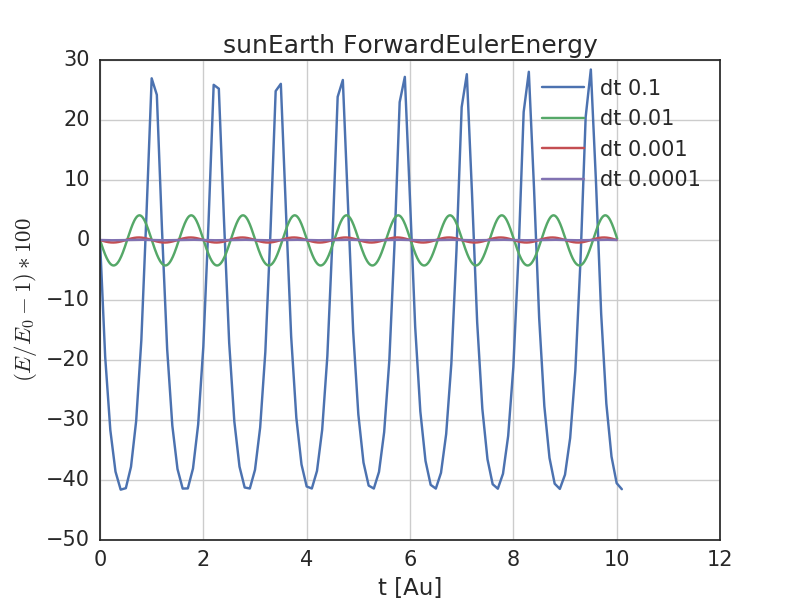
\includegraphics[width=0.99\textwidth]{/home/karl/doc/subj/att/fys4150/project3/resultsKeep/plots/sunEarthEnergyForwardEuler.png}
		\caption{Sun-Earth system. Total Energy divided by total energy first time step. Forward Euler. 10 years. \\ \textit{Energy is not preserved with the Forward Euler method}}
		\label{1}
	\end{figure}
\end{minipage}\hfill
\begin{minipage}{.49\textwidth} 
	\begin{figure}[H]
		\centering
		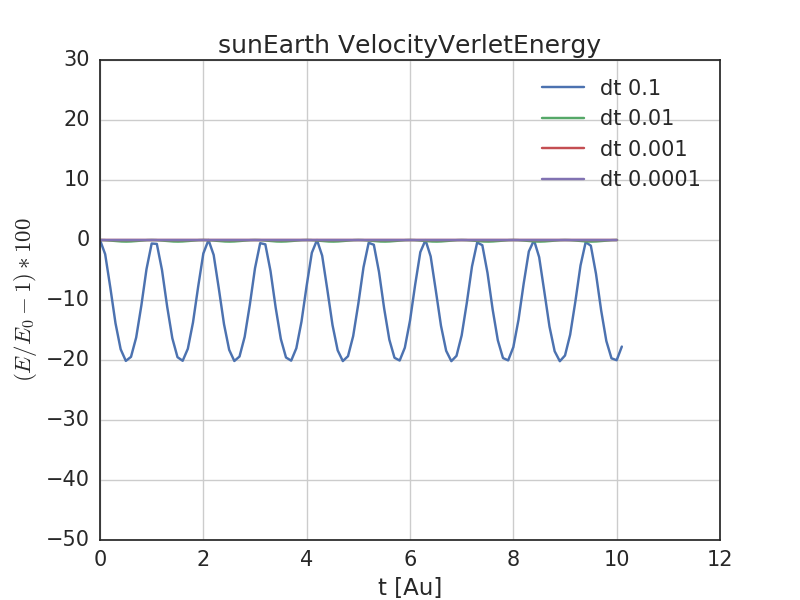
\includegraphics[width=0.99\textwidth]{/home/karl/doc/subj/att/fys4150/project3/resultsKeep/plots/sunEarthEnergyVelocityVerlet.png}
		\caption{Sun-Earth system. Total Energy divided by total energy first time step. Velocity Verlet. 10 years. \\ \textit{Energy is preserved in Velocity Verlet provided fine enough time step. }}
		\label{1}
	\end{figure}
\end{minipage}\hfill
\vspace{2ex}

The two figures above show that for forward Euler, energy can actually increase, even for smaller $\Delta t$. For Velocity Verlet, energy seems to be preserved faster compared to Forward Euler. Also, Velocity Verlet never make energy, as is the case for Forward Euler.\\

The next figure shows the same kind of figures as for energy above, but now for angular momentum. DO: Write why angular momentum is preserved.



\begin{minipage}{.49\textwidth} 
	\begin{figure}[H]
		\centering
		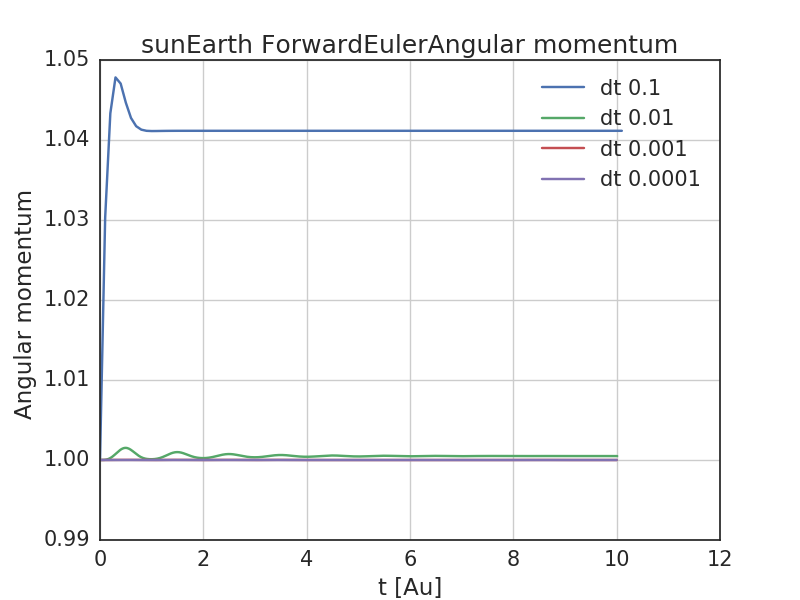
\includegraphics[width=0.99\textwidth]{/home/karl/doc/subj/att/fys4150/project3/resultsKeep/plots/sunEarthAngularMomentumForwardEuler.png}
		\caption{Sun-Earth system. Angular momentum divided by angular momentum first time step. Forward Euler. 10 years. \\ \textit{Angular momentum seems to be conserverd for the finest time step.}}
		\label{1}
	\end{figure}
\end{minipage}\hfill
\begin{minipage}{.49\textwidth} 
	\begin{figure}[H]
		\centering
		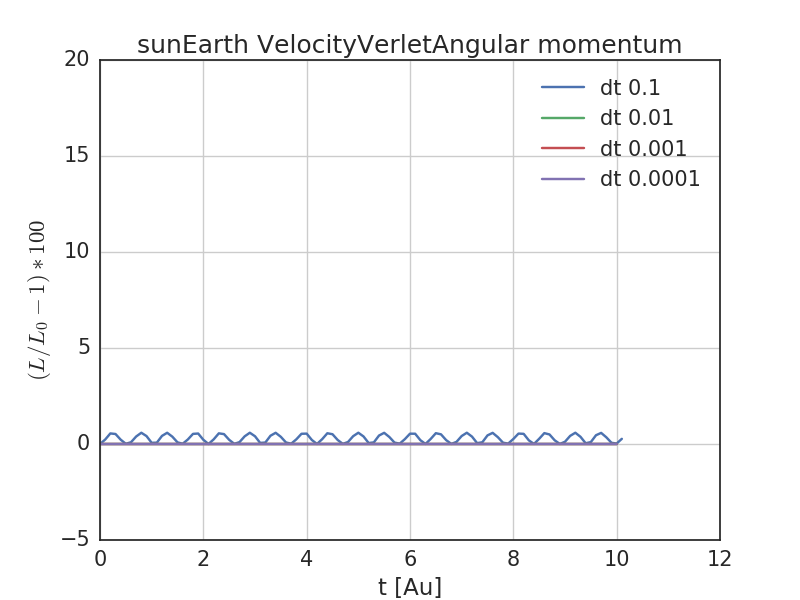
\includegraphics[width=0.99\textwidth]{/home/karl/doc/subj/att/fys4150/project3/resultsKeep/plots/sunEarthAngularMomentumVelocityVerlet.png}
		\caption{Sun-Earth system. Angular momentum divided by angular momentum first time step. Velocity Verlet. 10 years. \\ \textit{Angular momentum is conserverd given suffiently fine time steps. Conservation achieved faster than with Forward Euler.}}
		\label{1}
	\end{figure}
\end{minipage}\hfill
\vspace{2ex}

The figures above show that as $\delta t$ gets low, angular momentum is preserved. ALso, Velocity Verlet seems to give good angular momentum approximations compared to Forward Euler.\\

Since we know the exact solution for energy and angular momentum, or more precisely, the exact solution for the change, we have constructed a norm measure for computing convergence rates of the schemes. The error-norm is the supremum of the largest difference in energy compared to initial energy. The below figures show the results. DO: Write what to expect of these norms. We have truncation estimate for velocity and position, so it should just be to insert this into energy equation.

\begin{minipage}{.49\textwidth} 
	\begin{figure}[H]
		\centering
		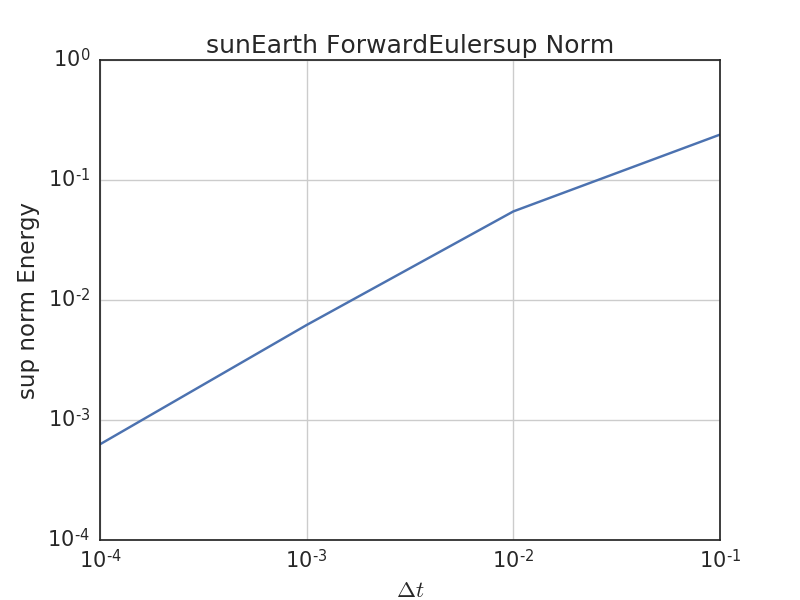
\includegraphics[width=0.99\textwidth]{/home/karl/doc/subj/att/fys4150/project3/resultsKeep/plots/sunEarthsupNormForwardEuler.png}
		\caption{Sun-Earth system. Sup-norm total energy. Forward Euler. \\ \textit{Forward Euler's sup-norm goes like $\mathcal{O}(\Delta t)$}}
		\label{1}
	\end{figure}
\end{minipage}\hfill
\begin{minipage}{.49\textwidth} 
	\begin{figure}[H]
		\centering
		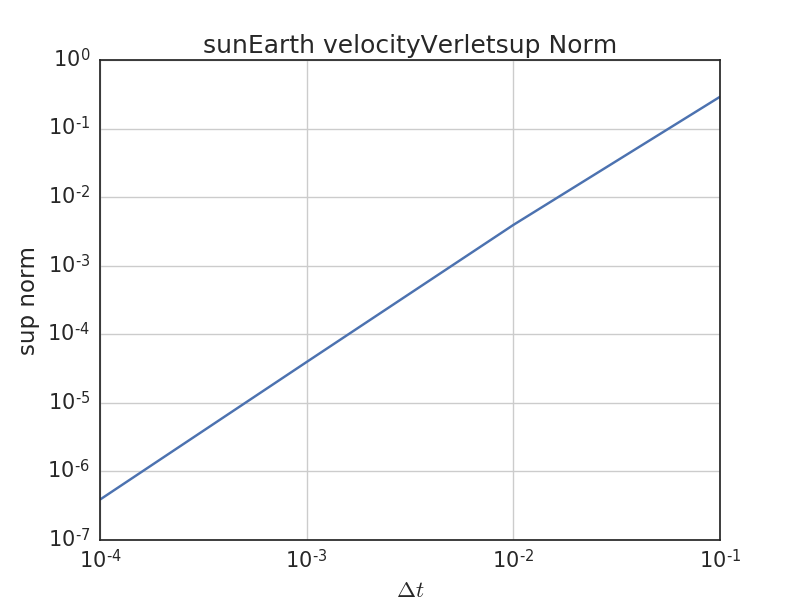
\includegraphics[width=0.99\textwidth]{/home/karl/doc/subj/att/fys4150/project3/resultsKeep/plots/sunEarthsupNormVelocityVerlet.png}
		\caption{Sun-Earth system. Sup-norm total energy. Velocity Verlet \\ \textit{The sup-norm in energy for Velocity Verlet goes one higher order than Forward Euler}}
		\label{1}
	\end{figure}
\end{minipage}\hfill
\vspace{2ex}

The above two figures shows that the error goes as 1st order for Forward Euler, while Velocity Verlet goes like 2nd order. DO: How does this compare to expectations?\\

In the same manner as for the energy-norms above, we have also constructed a norm for angular momentum. DO: What to expect. The below figure displays the results for the angular momentum norms.

\begin{minipage}{.49\textwidth} 
	\begin{figure}[H]
		\centering
		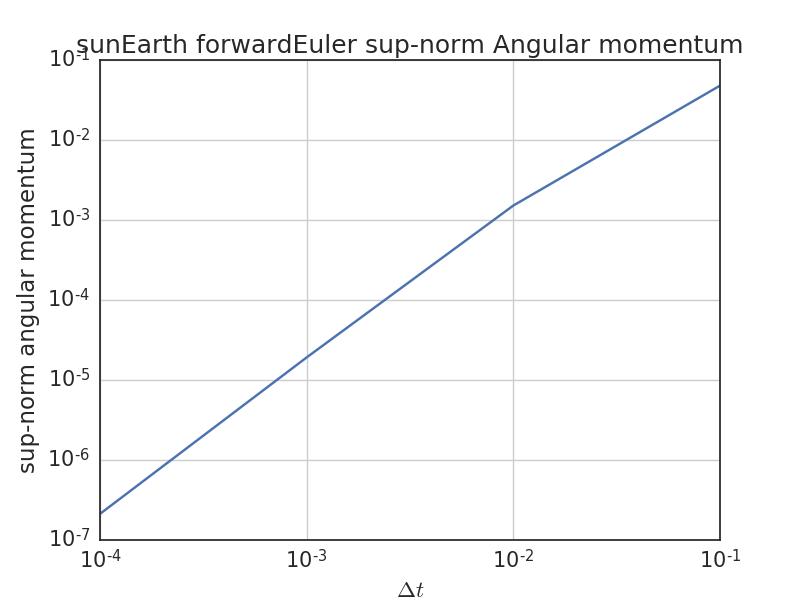
\includegraphics[width=0.99\textwidth]{/home/karl/doc/subj/att/fys4150/project3/resultsKeep/plots/sunEarthsupNormAngularMomentumForwardEuler.png}
		\caption{Sun-Earth system. Sup-norm Angular Momentum. Forward Euler \\ \textit{Forward Euler's sup-norm for angular momentum goes like $\mathcal{O}(\Delta t^2)$}.}
		\label{1}
	\end{figure}
\end{minipage}\hfill
\begin{minipage}{.49\textwidth} 
	\begin{figure}[H]
		\centering
		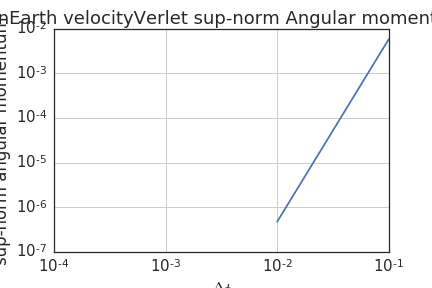
\includegraphics[width=0.99\textwidth]{/home/karl/doc/subj/att/fys4150/project3/resultsKeep/plots/sunEarthsupNormAngularMomentumVelocityVerlet.png}
		\caption{Sun-Earth system. Sup-norm Angular momentum. Velocity Verlet \\ \textit{Velocity Verlet's sup-norm error less than $10^{-12}$ like $\mathcal{O}(\Delta t^4)$.}}
		\label{1}
	\end{figure}
\end{minipage}\hfill
\vspace{2ex}

The two figures above shows that also for angular momentum, the order of the error-norm is higher for Velocity Verlet compared to Forward Euler, but now the difference is of order two. Also we see that the orders are doubled from the energy norms. DO: Comment on why higher order than energy, and how the results compare to expectations.\\

Knowledge about a methods correctness, discussed above, is crucial, but efficiency is also important. DO: FLOP-count for Forward-Euler and Velocity Verlet. The below figures show the computation time for the methods, forard Euler to the left and Velocity Verlet to the right.

\begin{minipage}{.49\textwidth} 
	\begin{figure}[H]
		\centering
		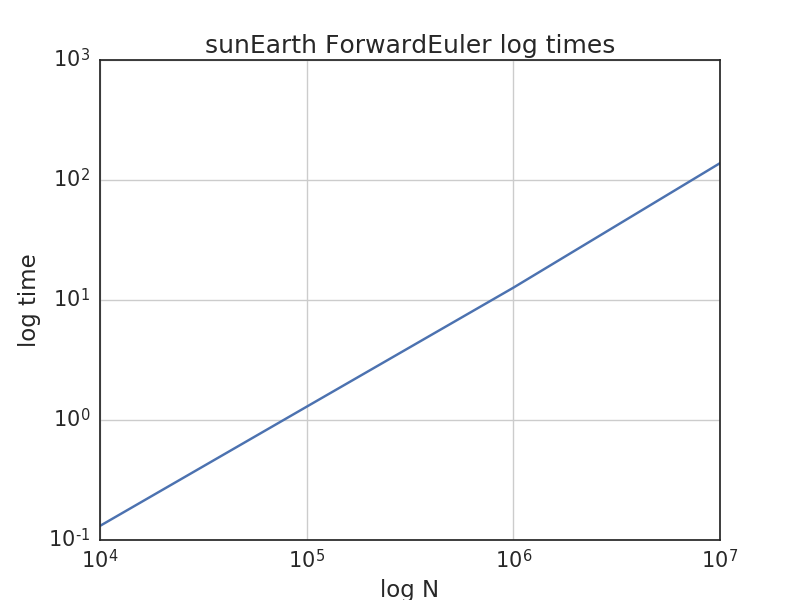
\includegraphics[width=0.99\textwidth]{/home/karl/doc/subj/att/fys4150/project3/resultsKeep/plots/sunEarthlogTimeUsedForwardEuler.png}
		\caption{Sun-Earth system. Log time. Forward Euler \\ \textit{Forward Euler's $\mathcal{O}(N)$}.}
		\label{1}
	\end{figure}
\end{minipage}\hfill
\begin{minipage}{.49\textwidth} 
	\begin{figure}[H]
		\centering
		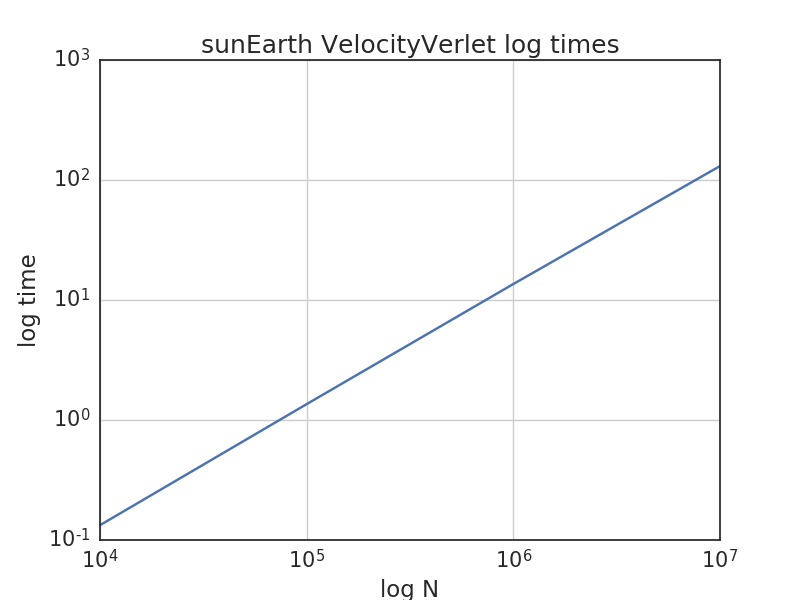
\includegraphics[width=0.99\textwidth]{/home/karl/doc/subj/att/fys4150/project3/resultsKeep/plots/sunEarthlogTimeUsedVelocityVerlet.png}
		\caption{Sun-Earth system. Log time. Velocity Verlet \\ \textit{Velocity Verlet's log time is of the same order as Forward Euler.}}
		\label{1}
	\end{figure}
\end{minipage}\hfill
\vspace{2ex}

The two figures above show that the Forward Euler and the Velocity Verlet method both has solution times that is of order 1 in N. This is as expected. The difference in FLOPS between forward Euler and Velocity Verlet is...DO.


\subsection{Escape velocity}
Another test to see if the solver obeys the physical laws, is to check if the escape velocity is correct. The escape velcoity equals the velcoity where potential energy equals kinetic energy

\begin{subequations}
	\begin{align}
	E_k  &= E_p \\
	\frac{1}{2} m_E v_{Escape}^2&= \frac{G M_{Sun} M_E}{r_0}\\
	\rightarrow v_E&=\sqrt{\frac{2G M_{Sun} }{r_0}}\\
	&=\sqrt{\frac{2* 4 \pi^2 AU^3 }{AU yr^2}}\\
	&=2 \pi\sqrt{2}\frac{ AU }{yr}
	\end{align}
\end{subequations}

Based on the above equation, we expect the simulations to gove escape then $v > 2\pi \sqrt{2}$. The figures below show the results.

\begin{figure}[H]
	\centering
	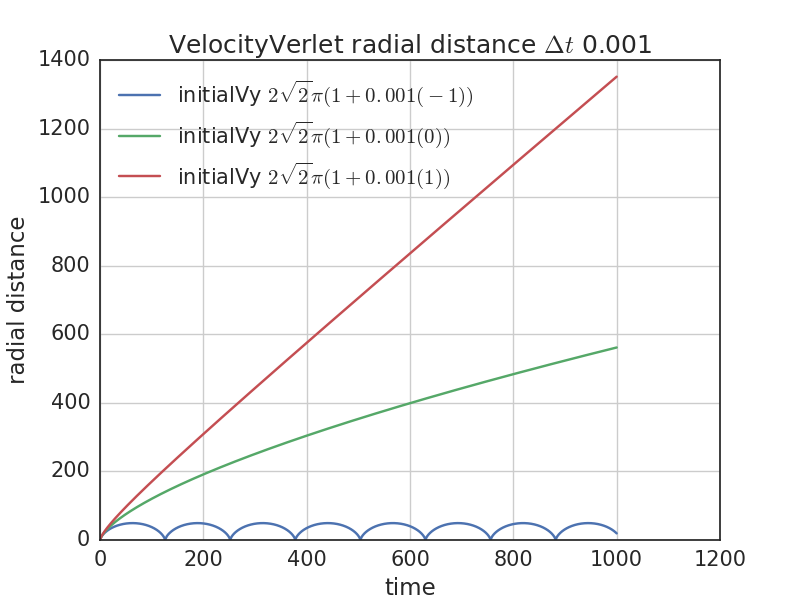
\includegraphics[width=0.6\textwidth]{/home/karl/doc/subj/att/fys4150/project3/resultsKeep/plots/sunEarthTerminalVelocityradialDistanceVelocityVerlet.png}
	\caption{Sun-Earth system. Escape valocity. Radial distance earth sun. \\ \textit{Escape for velocity equal to $0.1 \%$ of  $v = 2\sqrt{2}\pi$.}}
	\label{1}
\end{figure}



The figure above show that the simulated escape velocity is very close to the exact terminal velcocity, $2 \pi \sqrt{2}$, supporting the previous results indicating the validity of our solver as a good approximation method.\\

Another test, to see if the numerical solutions corresponds to analytical solutions, is to simulate the two planet system with different gravitational forces. DO: Write down a more general formula for the kinetic energy based on the revised forces.\\

The below figures show escapce velocities for the three different gravitational forces, all forces being lower than the standard force simulated above.


\begin{minipage}{.3\textwidth} 
	\begin{figure}[H]
		\centering
		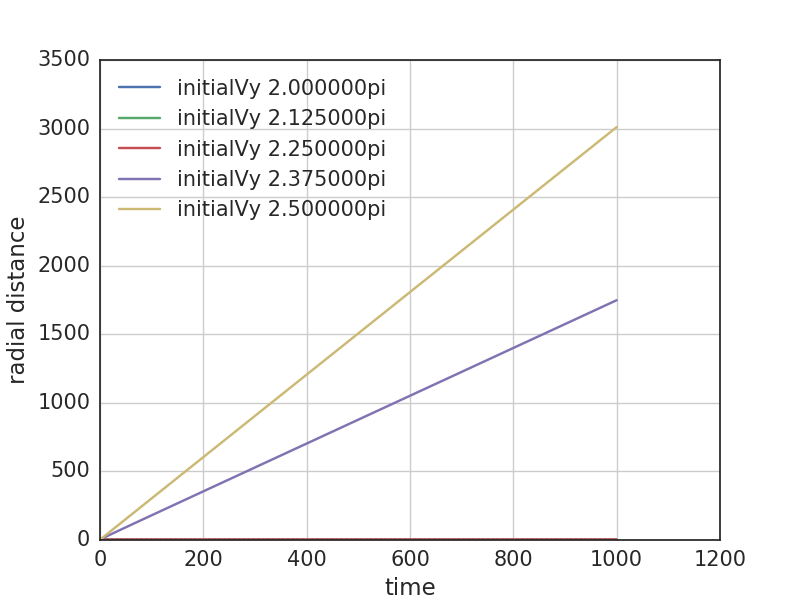
\includegraphics[width=0.99\textwidth]{/home/karl/doc/subj/att/fys4150/project3/resultsKeep/plots/sunEarthradialDistanceVelocityVerletbeta35.png}
		\caption{Sun-Earth system. Alternative force. Escape valocity. $\beta = 2.5$ \\ \textit{Escape velocity is reduced compared to case with normal gravititation.}}
		\label{1}
	\end{figure}
\end{minipage}\hfill
\begin{minipage}{.3\textwidth} 
	\begin{figure}[H]
		\centering
		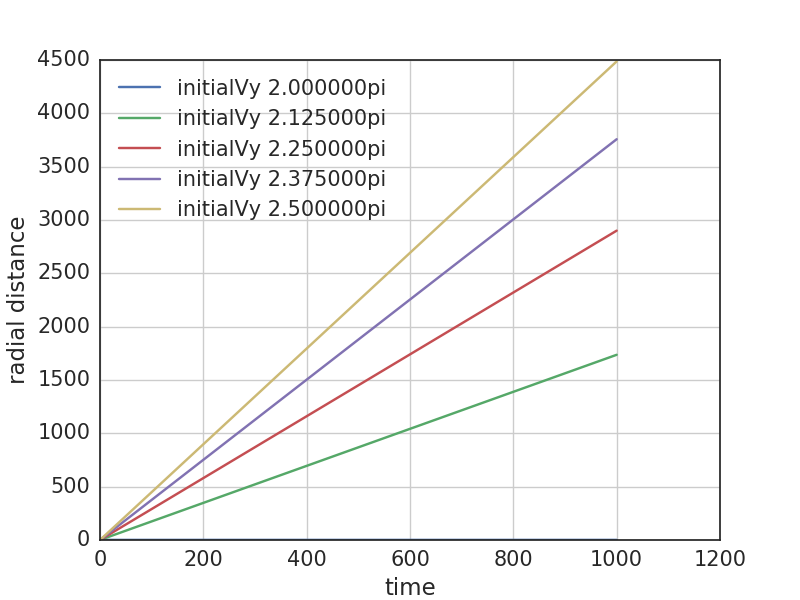
\includegraphics[width=0.99\textwidth]{/home/karl/doc/subj/att/fys4150/project3/resultsKeep/plots/sunEarthradialDistanceVelocityVerletbeta39.png}
		\caption{Sun-Earth system. Alternative force. Escape valocity. $\beta = 2.9$ \\ \textit{The escape velocity is further reduced, and seems to be closer to $2  \pi$}}
		\label{1}
	\end{figure}
\end{minipage}\hfill
\begin{minipage}{.3\textwidth} 
	\begin{figure}[H]
		\centering
		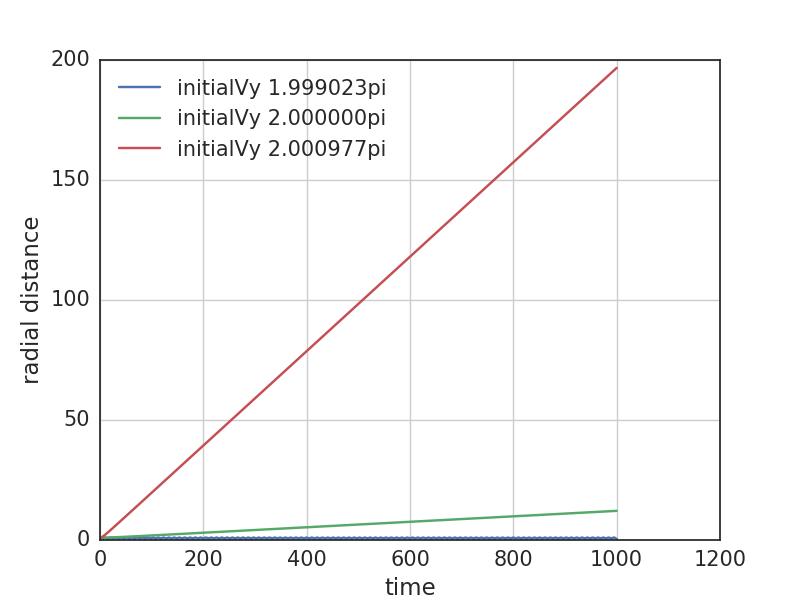
\includegraphics[width=0.99\textwidth]{/home/karl/doc/subj/att/fys4150/project3/resultsKeep/plots/sunEarthradialDistanceVelocityVerletbeta40.png}
		\caption{Sun-Earth system. Alternative force. Escape valocity. $\beta = 3.0$ \\ \textit{We get escape at $v = 2\pi$.}}
		\label{1}
	\end{figure}
\end{minipage}\hfill
\vspace{2ex}

The figures above show that the escape velocities are lowered when the gravitational forces are lowered. DO: Check agains thoretical expression. We see from the right most figure that the escape velocity is the same as the exact. DO: check the previous claim.

\subsection{Three planets}
Above we have seen that the solvers correspond well with expected behavoiur: Forward Euler does not preserve energy, while Velocity Verlet does, and basic exact results for escapce velocities, energy and angular momentum is well approximated. However, the above was only tested on a two-object system. To check whether the solver works for multibody systems, with more than two objects, a third planet, Jupiter, is added.\\

The figure below shows the orbits of the three body-system.

DO: Create and insert figures for 3 body non-moving sun here.\\

The figures above shows that the solver produces reasonable results for the three body system also. As for two bodies, the largest $\delta t$'s give bad approximations, while the smaller $\Delta t$'s give good approximations. DO: check the previous claim.\\

\subsection{Center of mass system}
All the above simulations were based on the assumption that the sun was stationary. This is not the case in reality. To make the  solver more realistic, we now introduce movement in the sun by letting the sun be modelled just as the other planets, gravity affecting also the sun's movement. \\

To make the plots easy to interpret, we make sure that the center of mass of the system is stationary. This we do by adjusting the initial velocity of the sun, utilizing the fact that the angular momentum of the system is preserved

\begin{subequations}
	\begin{align}
	0 &= \frac{d \vec R}{dt}	\\
	&= \frac{d}{dt} (\frac{1}{M} \sum_i^{Planets+Sun} m_i \vec{v}_i)\\
	&= \frac{1}{M} \sum_i^{Planets+Sun} m_i v_i \\
	\rightarrow 0 &=m_{sun} \vec{v}_{sun} + \sum_i^{Planets} m_i \vec{v}_i \\
	\vec{v}_{Sun} &= - \frac{\sum_i^{Planets} m_i \vec{v}_i}{m_{Sun}}
	\end{align}
\end{subequations}

The below figure shows the results with a moveing sun.\\

DO: Insert figure with moving sun and normal Jupiter mass here.\\

The figure above shows that the result of including movement in the sun is small. DO: Check the previous claim. To see how the program deals with a moving sun, we increase the mass of Jupiter. This should increase the movement of the sun, and make the results in the moving sun case different from the results in the stationary sun case. The results are shown in the figures below.\\

DO: Insert figures with increased mass of Jupiter, both for moving and non-moving sun.\\

The figures above show that when Jupiter's mass in increased, there is a signifiacant effect of introducing movement in the sun. The last figure also clearly shows that the center of mass remains fixed.


\subsection{Solar system}
The solver producing reasonable results for the three-body system, we are now ready to simulate the full solar system. Since we are using classes, going from three objects to ten objects constitutes nearly no work at all! We read in all planets from file in a loop, and use the same method as earlier for adding planets. That is all. The below figures displays the results for the full solar system, with a moving sun. \\

DO: Insert figure with solar system solutions here.\\

The above figure shows that the program nicely simulates the basic dynamics of the solar system. This is as expected, since the most significant forces are included in the program. 

\subsection{Perihelion precession}
Since the solver is working so well, we now want to try to reproduce the observed perihelion precession of Mercury by adding a relativistic gravitational term in the force on Mercury. Perihelion is the closest point between a planet and sun during one rotation. Over the period of a century, the position of Perhelion of Mercury is 43 arcsecconds. \\

We implement the relativistic term by creating a new class, "PlanetMercury", which inherits everything from the Planet class. Then we correct the acceleration function by overrideing it in the new class. We use only two objects for this simulation ,the sun and Mercury. Since the sun's mass is so much larger than the mass of Mercury, we solve this problem with a stationary sun. We saw that in the three body system, with larger planets than Mercury, the effect of introducing a moving sun was neglieble, so haivng a stationary sun in this scenario should not affect the results significantly. \\

We assume initial position of Mercury at perihelion, and localize perihelion at $(x,y) = (0.3075 Au, 0)$. Initial velocity is set to 12.44 $Au/Yr$. When doing this, we get the following results for the perihelion precession for different $\Delta t$.\\

DO: Insert table with preihelion precession and $\Delta t$.

DO: Comment on the results in the table above. 


\section{Conclusions}
In this project we solve problems for planetary motion, which mathematically are systems of 2nd order differential equations. To make the equations easier to work with, we scale the equations to astronomical units.\\

The systems of 2nd order equations are reformulated to systems of 1st order equations by use of variable substitution. \\

Solving the large system of equations in C++, we take apply classes and class inheritance.\\

Two numerical methods are used: the forward Euler method and the Velocity Verlet method. We show that the velocity Verlet method reproduces physical results like conservation of energy and angular momentum, while the Forward Euler method does not reproduce these results. The Velocity Verlet method converges faster to correct solutions, for preservation of energy and angular momentim, compared to the Forward Euler method. The velocity Verlet has twice the convergence rate of forward Euler when it comes to sup-norm in energy and angular momentum preservation, the velocity Verlet method being of order two and four for these quantitites respectively. Both methods gives bad results for the largest time steps. The methods are shown to involve approximatly the same amount of FLOPS.\\

The Velocity Verlet method reproduces the exact terminal velocity of a two object sun-earth system. Exact results are reproduced by Velocity Verlet also in scenarios where the gravitational force is changed. \\

Adding a third planet, Jupiter, to the stationary Sun earth system, gives reasonable results using Velocity Verlet: The orbits stay circular and stable. Also here the largest time steps give strange results, while the finer time steps gives convergent solutions. Making Jupiter's mass equal to the Sun's mass makes the earth escape. More realistic scenarios, that includes movement in the sun, keeping the center of mass of the system constant, produces reasonable results: When Jupiter's mass is enlarged, the sun starts to move. The center of mass is shown to be fixed.\\

The full solar system is simulated with the Velocity Verlet solver and with movement in the sun. The result seems reasonable, all orbits being stable.\\

By adding a relativistic correction to the gravitational force from sun on Mercury, the perihelion precession of Mercury around the sun is reproduced.\\

For future reference, we add the we could have improved the speed of the solvers by taking into account that the gravitational force between two planets are equal in magnitude. This implies that we could have halved the number of FLOPS!


\section{Feedback}
\subsection{Project 1}
This project has been extremely educational. We learned about about c++, especially pointers and dynamic memory allocoation. Also which for us was a well forgotten subject, we learned about dangerous of numerical round-off errors. \\

We feel the size of the project is large, much larger than typical assignments in other courses. However, the quality and quantity of the teaching without a doubt made the workload managable. The detailed lectures, combined with the fast and good respones on Piazza helped a lot!\\

We think the project could have gone even smoother, if we on the 2nd lab-session had learned basic branching in Github. We used a considerable amount of time finding out of this.\\

All in all, two thumbs up!

\subsection{Project 2}
\begin{itemize}
	\item  catch: We ended up using a lot of time making this work properly. Still we have some problems with catch and Qt. We think we might had benefited from a demonstration at the lab.
	
	\item We were not able to understand the revised Sturm-Bisection algorithm from Barth et al.'s \cite{barth} paper on the revised Sturm-Bisection. 
	
	\item Apart from the small details above, we are very happy about this project. How would have thought linear algebra could be fun?!
\end{itemize}

\subsection{Project 3}
\begin{itemize}
	\item  Classes: Very useful!
\end{itemize}













\pagebreak
\begin{thebibliography}{9}
	\bibitem{barth} 
	Barth, Martin, Wilkinson (1967)
	Calculation of eigenvalues of a symmetric tridiagonal matrix by the method of bisection. \textit{Numeriche mathematik 9, 386 - 393 (1967)}
	
	\bibitem{MHJ} 
	Hjorth-Jensen, M.(2015)
	Computational physics. Lectures fall 2015. 
	\url{https://github.com/CompPhysics/ComputationalPhysics/tree/master/doc/Lectures}
	
	\bibitem{MHJProject2} 
	Hjorth-Jensen, M.(2017)
	Project 2, fys4150 2017.
	\url{https://github.com/CompPhysics/ComputationalPhysics/blob/master/doc/Projects/2017/Project2/pdf/Project2.pdf}
	
	\bibitem{kiusalaas} 
	Kiusalaas, J.(2013)
	Numerical Methods in Engineering with Python 3. 3rd edition.
	
	\bibitem{taut} 
	Taut, M. (1993)
	Two electrons in an external oscillator potential: Particular analytic solutions of a Coulomb correlation problem \textit{Phys. Rev. A 48, 3561 (1993).}
	
	


\end{thebibliography}


\end{document}
